% Figure 1.2: Number 27 in Different Bases
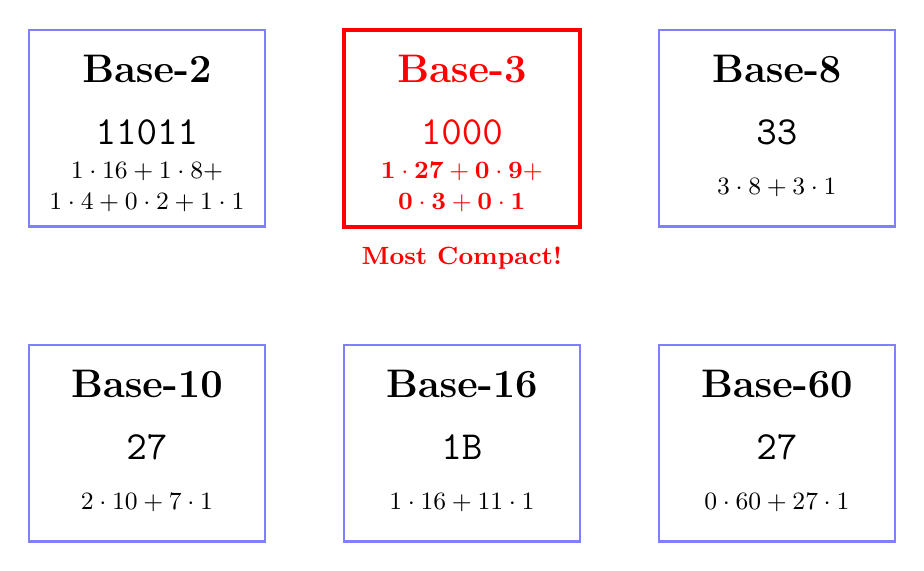
\begin{tikzpicture}[scale=1.0]

  % Title (implicit - will be in caption)

  % Base-2 (Binary)
  \node[font=\Large\bfseries] at (0,5) {Base-2};
  \node[font=\ttfamily\Large] at (0,4.2) {11011};
  \node[font=\small, align=center] at (0,3.5) {$1 \cdot 16 + 1 \cdot 8 +$\\$1 \cdot 4 + 0 \cdot 2 + 1 \cdot 1$};
  \draw[thick, draw=blue!50] (-1.5,3.0) rectangle (1.5,5.5);

  % Base-3 (Ternary) - highlighted
  \node[font=\Large\bfseries, red] at (4,5) {Base-3};
  \node[font=\ttfamily\Large, red] at (4,4.2) {1000};
  \node[font=\small, align=center, red] at (4,3.5) {$\mathbf{1 \cdot 27 + 0 \cdot 9 +}$\\$\mathbf{0 \cdot 3 + 0 \cdot 1}$};
  \draw[thick, draw=red, line width=1.5pt] (2.5,3.0) rectangle (5.5,5.5);
  \node[font=\small, red] at (4,2.6) {\textbf{Most Compact!}};

  % Base-8 (Octal)
  \node[font=\Large\bfseries] at (8,5) {Base-8};
  \node[font=\ttfamily\Large] at (8,4.2) {33};
  \node[font=\small, align=center] at (8,3.5) {$3 \cdot 8 + 3 \cdot 1$};
  \draw[thick, draw=blue!50] (6.5,3.0) rectangle (9.5,5.5);

  % Base-10 (Decimal)
  \node[font=\Large\bfseries] at (0,1.0) {Base-10};
  \node[font=\ttfamily\Large] at (0,0.2) {27};
  \node[font=\small, align=center] at (0,-0.5) {$2 \cdot 10 + 7 \cdot 1$};
  \draw[thick, draw=blue!50] (-1.5,-1.0) rectangle (1.5,1.5);

  % Base-16 (Hexadecimal)
  \node[font=\Large\bfseries] at (4,1.0) {Base-16};
  \node[font=\ttfamily\Large] at (4,0.2) {1B};
  \node[font=\small, align=center] at (4,-0.5) {$1 \cdot 16 + 11 \cdot 1$};
  \draw[thick, draw=blue!50] (2.5,-1.0) rectangle (5.5,1.5);

  % Base-60 (Babylonian)
  \node[font=\Large\bfseries] at (8,1.0) {Base-60};
  \node[font=\ttfamily\Large] at (8,0.2) {27};
  \node[font=\small, align=center] at (8,-0.5) {$0 \cdot 60 + 27 \cdot 1$};
  \draw[thick, draw=blue!50] (6.5,-1.0) rectangle (9.5,1.5);

\end{tikzpicture}
